\section{Exercise 3.1}
\subsection{Request}
Find the overall collision resolution efficiency $\eta$ in the different cases in which the initial frame size is set to r1=1,2,3,4,5,6.
\subsection{Data}
\begin{itemize}
\item $r_1$ = 1, 2, 3, 4, 5, 6
\item $L_2$ = 4
\item $L_3$ = 51/8
\end{itemize}
\subsection{Solution}
To compute the $\eta$ in the different cases we can use the formula:

\begin{equation}
\eta = \frac{N} {L_N}
\end{equation}

So we need to calculate first $L_4$ in all the six cases required by the exercise. We can do it using the reported formula:

\begin{equation}
L_4^* = r_1 + P(S=0) \cdot L_4 + P(S=1) \cdot L_3 + P(S=2) \cdot L_2 + P(S=3) \cdot L_1
\end{equation}

\subsubsection{Probabilities}
In order to solve this equation we need to calculate all the probabilities in the six cases:
\begin{itemize}
\item $r_1 = 1$
\begin{equation}
P(S=0) = 1
\end{equation}
\begin{equation}
P(S=1) = P(S=2) = P(S=3) = P(S=4) = 0
\end{equation}
All the 4 tags must choose the single existing slot.

\item $r_1 = 2$
\begin{equation}
P(S=0) = (\frac{1}{2})^4 \cdot 2 +  (\frac{1}{2})^4 \cdot \binom{4}{2} \cdot \frac{2}{2} = \frac{1}{2}
\end{equation}
\begin{equation}
P(S=1) = (\frac{1}{2})^4 \cdot 4 \cdot 2 = \frac{1}{2}
\end{equation}
\begin{equation}
P(S=2) = P(S=3) = P(S=4) = 0
\end{equation}

\item $r_1 = 3$
\begin{equation}
P(S=0) = (\frac{1}{3})^4 \cdot 3 +  (\frac{1}{3})^4 \cdot \binom{4}{2} \cdot \frac{2 \cdot 3}{2} = \frac{7}{27}
\end{equation}
\begin{equation}
P(S=1) = (\frac{1}{3})^4 \cdot \binom{4}{1} \cdot 3 \cdot 2 = \frac{8}{27}
\end{equation}
\begin{equation}
P(S=2) = (\frac{1}{3})^4 \cdot 4 \cdot 3 \cdot 3 \cdot 2 \cdot \frac{1}{2} = \frac{4}{9}
\end{equation}
\begin{equation}
P(S=3) = P(S=4) = 0
\end{equation}

\item $r_1 = 4$
\begin{equation}
P(S=0) = (\frac{1}{4})^4 \cdot 4 +  (\frac{1}{4})^4 \cdot \binom{4}{2} \cdot 4 \cdot 3 \cdot \frac{1}{2} = \frac{5}{32}
\end{equation}
\begin{equation}
P(S=1) = (\frac{1}{4})^4 \cdot 4 \cdot 4 \cdot 3 = \frac{3}{16}
\end{equation}
\begin{equation}
P(S=2) = (\frac{1}{4})^4 \cdot 4 \cdot 4 \cdot 3 \cdot 3 \cdot 2 \cdot \frac{1}{2} = \frac{9}{16}
\end{equation}
\begin{equation}
P(S=3) = 0
\end{equation}
\begin{equation}
P(S=4) = (\frac{1}{4})^4 \cdot 4 \cdot 4 \cdot 3 \cdot 2 \cdot 1 = \frac{3}{32}
\end{equation}

\item $r_1 = 5$
\begin{equation}
P(S=0) = (\frac{1}{5})^4 \cdot 5 +  (\frac{1}{5})^4 \cdot \binom{4}{2} \cdot 5 \cdot 4 \cdot \frac{1}{2} = \frac{13}{125}
\end{equation}
\begin{equation}
P(S=1) = (\frac{1}{5})^4 \cdot 4 \cdot 5 \cdot 4 = \frac{16}{125}
\end{equation}
\begin{equation}
P(S=2) = (\frac{1}{5})^4 \cdot 4 \cdot 5 \cdot 3 \cdot 4 \cdot 3 \cdot \frac{1}{2} = \frac{72}{125}
\end{equation}
\begin{equation}
P(S=3) = 0
\end{equation}
\begin{equation}
P(S=4) = (\frac{1}{5})^4 \frac{5!}{(5-4)!} = \frac{24}{125}
\end{equation}

\item $r_1 = 6$
\begin{equation}
P(S=0) = (\frac{1}{6})^4 \cdot 6 +  (\frac{1}{6})^4 \cdot \binom{4}{2} \cdot 6 \cdot 5 \cdot \frac{1}{2} = \frac{2}{27}
\end{equation}
\begin{equation}
P(S=1) = (\frac{1}{6})^4 \cdot 4 \cdot 6 \cdot 5 = \frac{5}{54}
\end{equation}
\begin{equation}
P(S=2) = (\frac{1}{6})^4 \cdot 4 \cdot 6 \cdot 3 \cdot 5 \cdot 4 \cdot \frac{1}{2} = \frac{5}{9}
\end{equation}
\begin{equation}
P(S=3) = 0
\end{equation}
\begin{equation}
P(S=4) = (\frac{1}{6})^4 \frac{6!}{(6-4)!} = \frac{5}{18}
\end{equation}
\end{itemize}

Now we can calculate the value of $L_4$:
\begin{equation}
\begin{split}
L_4 & = 4 + \sum_{i=0}^{3} P(S=i) \cdot L_{4-i} = \\
& = 4 + P(S=0) \cdot L_4 + P(S=1) \cdot L_3 +  P(S=2) \cdot L_2 +  P(S=3) \cdot L_1 = \\
& = 4 + \frac{5}{32} \cdot L_4 + \frac{3}{16} \cdot L_3 + \frac{9}{16} \cdot L_2 + 0 \\ \\
L_4 & = \frac{4 + \frac{3}{16} \cdot L_3 + \frac{9}{16} \cdot L_2}{1 - \frac{5}{32}} = \frac{953}{108}
\end{split}
\end{equation}

Now we can calculate the values of $L_4^*$ in the six requested cases, once computed them we can calculate the overall collision resolution efficiency $\eta$ for each case.

\begin{itemize}
\item $r_1 = 1$
\begin{equation}
\begin{split}
L_4^* & = 1 + 1 \cdot L_4 = \frac{1061}{108} \simeq 9,824 \\
\eta_1 & = 0,407
\end{split}
\end{equation}

\item $r_1 = 2$
\begin{equation}
\begin{split}
L_4^* & = 2 + \frac{1}{2} \cdot L_4 + \frac{1}{2} \cdot L_3 = \frac{4147}{432} \simeq 9,600 \\
\eta_2 & = 0,417
\end{split}
\end{equation}

\item $r_1 = 3$
\begin{equation}
\begin{split}
L_4^* & = 3 + \frac{7}{27} \cdot L_4 + \frac{8}{27} \cdot L_3 + \frac{4}{9} \cdot L_2 \simeq 8,954 \\
\eta_3 & = 0,447
\end{split}
\end{equation}

\item $r_1 = 4$
\begin{equation}
\begin{split}
L_4^* & = 4 + \frac{5}{32} \cdot L_4 + \frac{3}{16} \cdot L_3 + \frac{9}{16} \cdot L_2 = \frac{953}{108} \simeq 8,824 \\
\eta_4 & = 0,453
\end{split}
\end{equation}

\item $r_1 = 5$
\begin{equation}
\begin{split}
L_4^* & = 5 + \frac{13}{125} \cdot L_4 + \frac{16}{125} \cdot L_3 + \frac{72}{125} \cdot L_2 \simeq 9,038 \\
\eta_5 & = 0,443
\end{split}
\end{equation}

\item $r_1 = 6$
\begin{equation}
\begin{split}
L_4^* & = 6 + \frac{2}{27} \cdot L_4 + \frac{5}{54} \cdot L_3 + \frac{5}{9} \cdot L_2 \simeq 9,466 \\
\eta_6 & = 0,423
\end{split}
\end{equation}
\end{itemize}

\section{Exercise 3.2}

\begin{figure}[H]
    \centering
    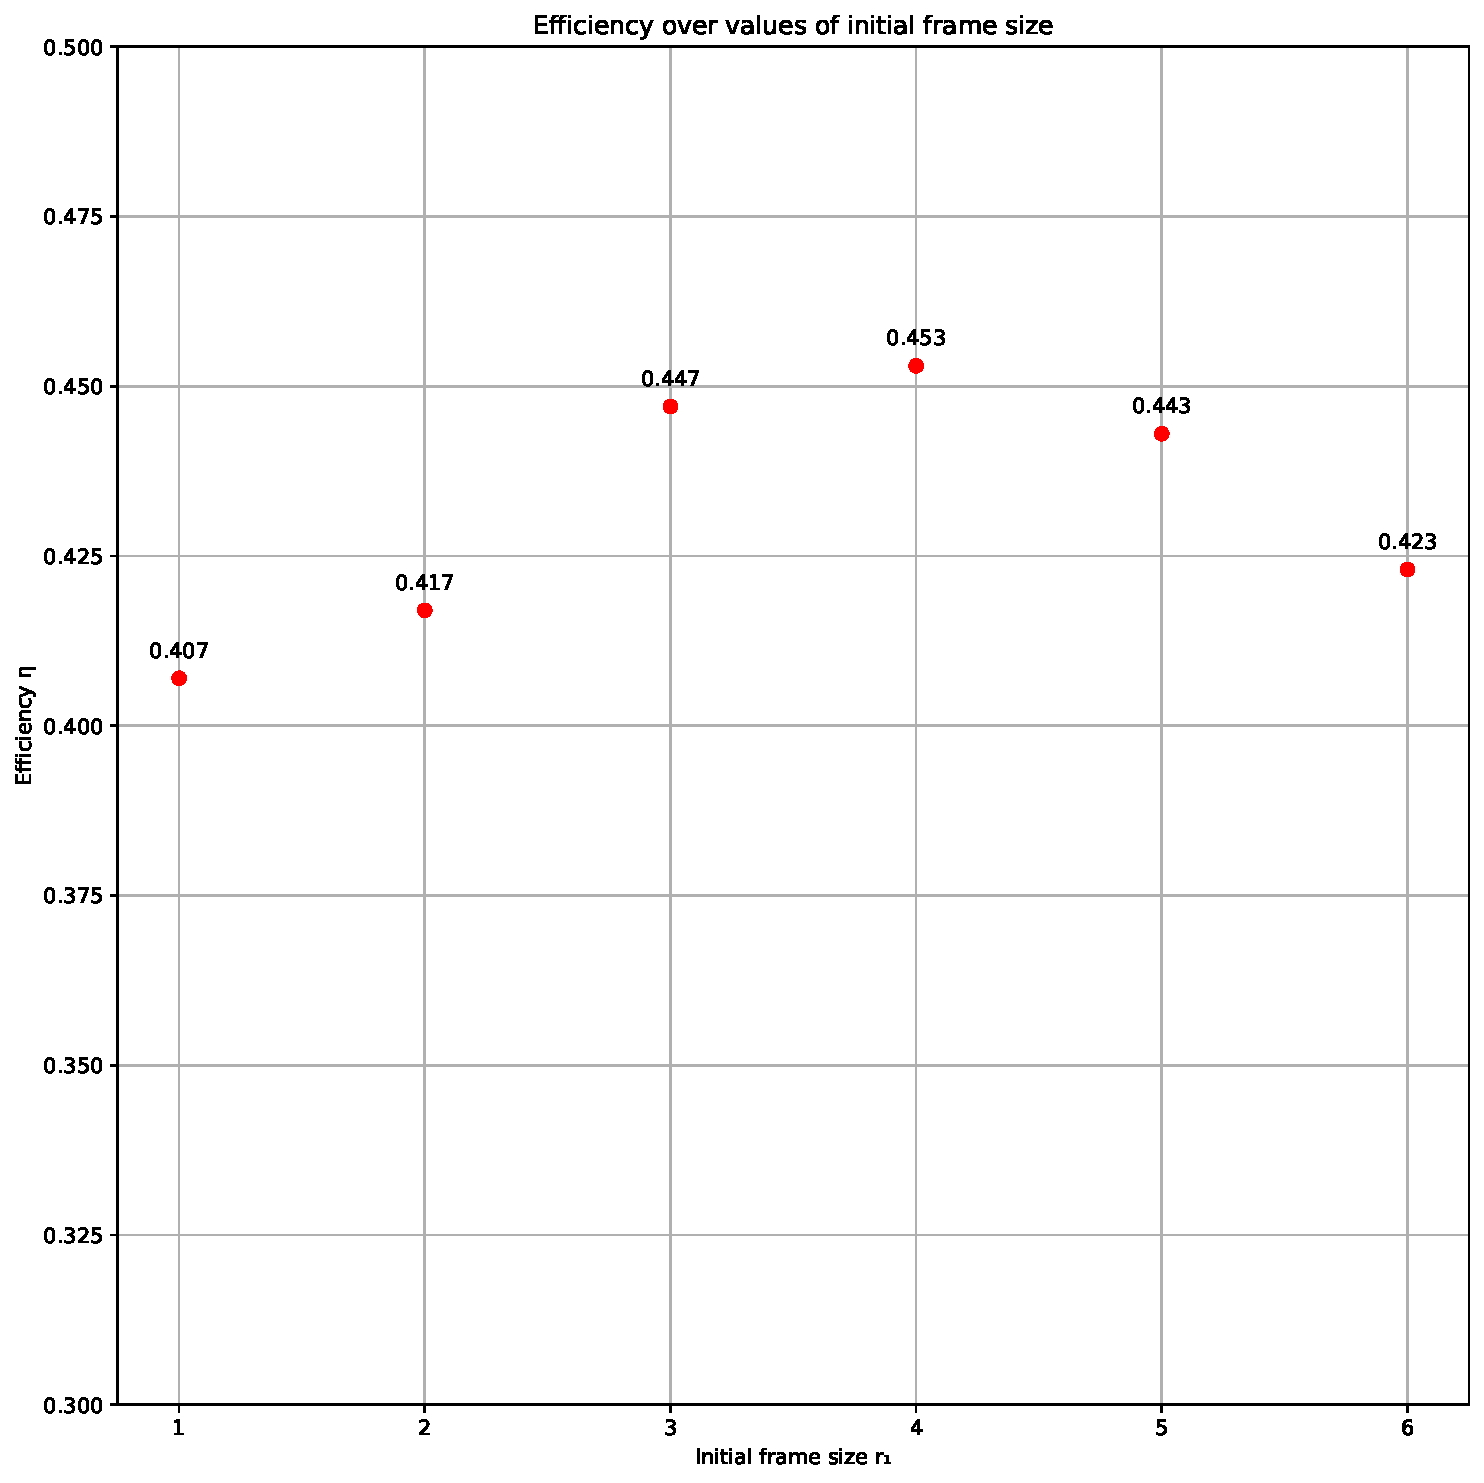
\includegraphics[width=\linewidth, keepaspectratio]{Graph.pdf}
    \caption{Exercise 3.2 plot}
\end{figure}

\section{Exercise 3.3}
The maximum value of efficiency, denoted by $\eta$, is observed when the initial frame size is $r_1 = 4$. \\
This result aligns well with theoretical expectations, which predict that the highest efficiency is achieved when the frame size matches the number of tags, i.e., when $r_1 = N$.

When $r_1$ is smaller than N, the number of available slots is insufficient to accommodate all tags without contention, resulting in a high number of collisions and, consequently, a lower efficiency. On the other hand, when $r_1$ is larger than N, the frame includes more slots than necessary, leading to an increased number of empty slots. These unused slots do not contribute to successful transmissions and thus reduce the overall efficiency.

Therefore, the optimal value of $r_1$ represents a trade-off that minimizes collisions while avoiding excessive empty slots, which is precisely achieved when $r_1$ equals the number of tags N.
